\documentclass{article}
\usepackage[utf8]{inputenc}
\usepackage{hyperref}

\begin{document}

\section{Description and relevance for the HL-LHC}

Unlike other sectinos of this document, ``data science tools'' is not an experiment or software product with centralized management. The word describes a collection of interrelated small projects, developed by a network of teams or individuals in different organizations and communities. It is relevant to HL-LHC planning because many of the developers and users of this software are LHC physicists, particularly the Ph.D.\ students and postdocs involved in the actual implementation of LHC analyses.

We use the word ``data science'' for two reasons. The first reason is that most of the foundational software underlying this work was developed by cross-disciplinary scientists (i.e.\ not just HEP) and by statistician-programmers in industry: business intelligence, finance, web analytics, and other fields that require timely calculations on large datasets---collectively known as ``data science.'' The second reason is that the culture of distributed software development that is taking hold in HEP derives from exposure to a similar culture in the data science industry. The norms are changing: it has become more common for developers to contribute to a variety of related projects, not just their own, and to value fine-grained packaging in an interoperable ecosystem.

Although many of the data science-based projects in HEP are self-motivated---physicists spontaneously writing software to fulfill the needs of their own analyses---we can't simply ignore such developments and assume that it will all work out in the end. Since the rise of open-source software in the late 1990's/early 2000's, the decentralized nature of its development has been in tension with business needs for stability, reliable planning, and influence over the direction of development---just as we need to prepare for the HL-LHC a decade in advance. In fact, it's somewhat surprising that this ``chaotic'' model of software development works at all, but, crucially, 20~years of experience has shown that it does. A ``tragedy of the commons'' does not apply because software is not a scarce resource like grazing pasture---it can't be used up by a corporation taking it without recompense. Moreover, communal software development provides its own incentive for support. Software products are moving targets: if stakeholders do not contribute their own modifications to the ever-changing community version, they risk having to maintain an unmergeable fork. All of this has led to the remarkable situation in which billion dollar companies now contribute to data analysis software that is available for free.

The relevance of this to the HL-LHC is that our scientific goals are also a specialized interest, and we can either influence these shared software products to meet our needs or we will have to maintain our own software stacks. To an extent, young physicists (i.e.\ graduate students and postdocs) are making this decision for us by adopting data science software in their analyses and contributing back to it, as well as developing their own packages to satisfy HEP-specific needs. This has been a clear trend in the past 3--4~years, with community support and the emergence of community projects. We can support this work by connecting it to (not absorbing it into) established HEP products like ROOT and the LHC experiment frameworks, and by mediating communication so that these small-granularity software products can each find their niche, and only one per niche. We can also steer the grassroots efforts in a forward-looking direction: physicists may be developing tools that suit their own analyses now, but will they scale to HL-LHC luminosities?

Data science software in HEP is a side job for many of its developers, for whom a physics analysis or a thesis is the top priority. That makes it particularly vulnerable---the immediate need to get a physics project done quickly very often outweighs the future need to get projects like it done in a better way. Git history is littered with abandoned projects such as these. On the other hand, the will to develop such software is already present in the community---we don't have to convince anybody to do it---we just need to ensure that it grows in the right direction.

\section{The HEP analysis software landscape is changing}

Although we can find evidence of physicists attempting to use tools like NumPy, SciPy, Matplotlib, Pandas, Hadoop, and Spark over the past 15--20 years, these data science tools have only become a major part of HEP analysis in the past 4--5 years. Causes for this change are hard to identify conclusively because it is a bottom-up movement, but the following are likely influences:

\begin{itemize}
\item Externally, data analysis tools have consolidated on Python and array-oriented programming. The landscape had previously been more fractured: in the early 2000's, novel statistical techniques were implemented in R and big datasets were managed by Java, but in the past 5~years, Python has become the common language for both. Because of these changes in the industry, young physicists are much more likely to see Python in university courses and code examples on the web, and a career path that involves Python expertise is more attractive than one without. Keep in mind that ``the industry'' is orders of magnitude larger than HEP, and many physics students are at least considering careers outside of HEP. A significant fraction of the newcomers to our field have prior experience with Python and have good reason to want more.

\item Internally, organizations within HEP have mediated communications about data science software, helping physicist-developers find each other, reduce duplication, and build on each others' tools. These organizations have legitimized the idea of using data science software in HEP, and they are actively supporting its development, especially for the foundational components that enable specialized tools.
\end{itemize}

The first of these organizations, the \href{https://hepsoftwarefoundation.org/}{HEP Software Foundation (HSF)}, was conceived in a community event at SLAC in 2015 and cohered in the \href{https://hepsoftwarefoundation.org/organization/cwp.html}{Community Whitepaper project} of 2017. The HSF's primary mission is communication: helping project developers find each other to work toward a common vision, as well as providing fora in which new projects are conceived, particularly across experiment boundaries. The HSF does not fund projects or direct them. The \href{https://hepsoftwarefoundation.org/workinggroups/dataanalysis.html}{Data Analysis Working Group (DAWG)} hosts monthly meetings on data analysis software, giving physicist-developers a place to showcase their work and find users and collaborators.

The \href{https://hepsoftwarefoundation.org/workinggroups/pyhep.html}{``Python in HEP'' working group (PyHEP)} hosts large, annual workshops on both domain-specific and infrastructure libraries, as well as Python Module of the Month meetings to focus on data science and HEP domain-specific packages of interest.

\href{http://diana-hep.org/}{DIANA/HEP} and its much larger successor, \href{https://iris-hep.org/}{IRIS-HEP}, were funded by the NSF in 2015 and 2018, respectively, to support the development of HEP software (a)~financially, by funding software developers, (b)~as an intellectual hub for sharing knowledge and fostering connections, and (c)~through training and eduation. The directly funded software products include Awkward Array, hist, pyhf, recast, ServiceX, SkyhookDM, Uproot, and Vector, all of which have substantially influenced the Python/data science ecosystem in HEP. Weekly DIANA/HEP and IRIS-HEP topical meetings are held by physicists and occasionally draw data scientists from industry to share tools and techniques, and IRIS-HEP hosts cross-experiment software tutorials, as well as the annual \href{http://codas-hep.org/}{CoDaS-HEP school}.

Other national projects, such as \href{https://gtr.ukri.org/projects?ref=ST\%2FV002562\%2F1}{SWIFT-HEP} in the U.K., are fulfilling a similar role to IRIS-HEP in the U.S.

Less formally, the \href{https://scikit-hep.org/}{Scikit-HEP} project (since 2017) has focused efforts to build a Pythonic ecosystem for analysis in HEP---the first to do so---by providing a common goal, brand, high standards of quality packaging, and a web presence. It grew dramatically, providing many of the packages listed above, with strong community adoption. The developers of software libraries like \href{https://coffeateam.github.io/coffea/}{Coffea}, \href{https://fast-hep.web.cern.ch/fast-hep/}{FAST-HEP}, \href{https://goofit.github.io/}{GooFit}, \href{https://iminuit.readthedocs.io/}{iminuit}, and \href{https://zfit.readthedocs.io/en/latest/}{zfit} also have a strong influence on the ecosystem, since each widely-used software package accretes a planetary system of related tools. Coffea, a Fermilab project that glues together foundational components and adds whatever is missing for analysis, has been particularly influential. It can be credited with the initial promotion of Awkward Array and it acts as a rapid testing ground for components that eventually spin off into their own infrastructure components, such as hist (for histograms) and Vector (for Lorentz vectors).

The big picture of developments in data science software, HEP software, and the LHC/HL-LHC timeline are depicted together in Figure~\ref{fig:hllhc-python-timeline-paper}. Major developments in data science---scientific Python, big data, GPUs and machine learning---roughly coincide with the development and first run of the LHC, from the late 1990's to 2015. The HSF, DIANA/HEP, and IRIS-HEP were active after 2015, and these organizations fostered the development of data science-oriented software in HEP.

\begin{figure}
% 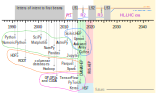
\includegraphics[width=\linewidth]{fig/hllhc-python-timeline-paper.pdf}

\caption{Timeline of developments in scientific Python (dashed green outline), big data (orange), GPUs and machine learning (magenta), and data science in HEP (blue), overlaid on the LHC, HL-LHC, HSF, DIANA/HEP, and IRIS-HEP timelines. \label{fig:hllhc-python-timeline-paper}}
\end{figure}

Originally, data science in industry was split between R for statistical techniques, Java for scale-out (particularly Hadoop and Spark), and Python. Figure~\ref{fig:analytics-by-language} shows the ascendancy of Python as the language of data analytics, as measured by Google search terms. By 2018, ``Python'' was more frequently searched with ``analytics'' than ``R'' or ``Java,'' and machine learning, which entered a renaissance in 2015, was Python-focused from the start.

\begin{figure}
% 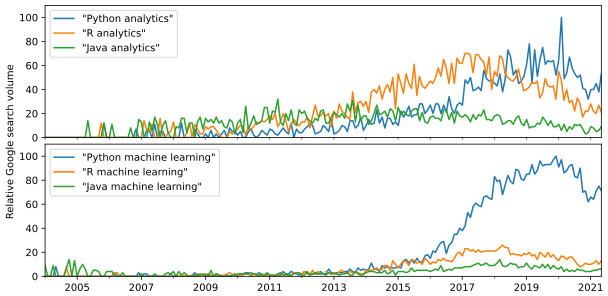
\includegraphics[width=\linewidth]{fig/analytics-by-language.pdf}

\caption{Relative Google search volume (from \href{https://trends.google.com/}{trends.google.com}) for ``Python,'' ``R,'' and ``Java'' in the same search string with ``analytics'' (top) and ``machine learning'' (bottom). \label{fig:analytics-by-language}}
\end{figure}

Within HEP, adoption of Python also ramped up in the years following 2015. As a specific illustration of this trend, Figure~\ref{fig:lhlhc-github-languages-paper} shows the language of GitHub repositories created by CMS physicists, where CMS physicists are identified as users who forked {\tt cms-sw/cmssw} (\href{https://github.com/jpivarski-talks/2021-02-24-reload-statistics}{link to full analysis}). Python usage has been steadily growing and surpassed C++ in 2019. GitHub's language assignment is exclusive---each repository is considered entirely Python or entirely C++, but in reality most are mixed---so we can investigate with more precision by counting repositories that match search terms, such as ``numpy,'' ``matplotlib,'' and ``pandas.'' In Figure~\ref{fig:lhlhc-github-overlay-lin-paper}, we see the use of these libraries steadily increasing (long before ``uproot''). Now they appear in repositories as often as ROOT-related terms, such as ``TFile'' and ``import ROOT'' (``from ROOT import'' is less common and highly correlated with the 3 ROOT-related terms shown on the plot).

\begin{figure}
% \includegraphics[width=\linewidth]{fig/lhlhc-github-languages-paper.pdf}

\caption{Number of GitHub repositories created by CMS physicists by language (exclusive categories), showing the rise of Python and Jupyter. CMS physicists are identified as users who fork {\tt cms-sw/cmssw}. HSF, DIANA/HEP, and IRIS-HEP timelines are overlaid (top-right). \label{fig:lhlhc-github-languages-paper}}
\end{figure}

\begin{figure}
% \includegraphics[width=\linewidth]{fig/lhlhc-github-overlay-lin-paper.pdf}

\caption{Number of GitHub repositories, created by CMS physicists (same analysis as in Figure~\ref{fig:lhlhc-github-languages-paper}), that match search strings (non-exclusive categories). This shows the rise of Pythonic data analysis (NumPy, Matplotlib, Pandas), with ROOT (C++ and Python, also increasing) for scale. \label{fig:lhlhc-github-overlay-lin-paper}}
\end{figure}

A pre-workshop survey of \href{https://indico.cern.ch/e/PyHEP2020}{PyHEP 2020} registrants also indicated that the HEP community is using an even mix of C++ and Python. Figure~\ref{fig:pyhep2020-survey-paper} shows responses to basic questins and Figure~\ref{fig:lhlhc-familiarity-with-packages-paper} shows the registrants' familiarity and usage of popular data science and HEP tools.

\begin{figure}
% \includegraphics[width=\linewidth]{fig/pyhep2020-survey-paper.pdf}

\caption{Survey results from 406 registrants of PyHEP 2020 illustrating the mix of C++ and Python (and no other language) among physicists, and the use of Python primarily for analysis. \label{fig:pyhep2020-survey-paper}}
\end{figure}

\begin{figure}
% \includegraphics[width=\linewidth]{fig/lhlhc-familiarity-with-packages-paper.pdf}

\caption{Familiarity and usage of data science tools (top) and HEP data analysis tools (bottom) from the same survey as Figure~\ref{fig:pyhep2020-survey-paper}. \label{fig:lhlhc-familiarity-with-packages-paper}}
\end{figure}

Clearly, HEP analysis culture is in the midst of a transition, perhaps as significant as the transition from Fortran to C++ and object oriented programming in the 1990's. The programming languages and software library choices plotted above are the most quantifiable aspects of this transition, but other changes are indicated by the words physicists use to describe their analysis or analysis software.

\begin{itemize}
\item HEP data analysts are becoming averse to monolithic frameworks. ``{\bf Framework}'' (or ``{\bf platform}'') used to be a more positive word: ROOT and collaboration software are self-described as frameworks, and even small analysis groups developed frameworks for their own ntuple's schemas. A framework, \href{https://root.cern.ch/root/htmldoc/guides/users-guide/ROOTUsersGuide.html#the-framework}{in this sense}, provides all the essentials in one package but requires users to fit their workflows into the application. Data science ``{\bf libraries}'' (or ``{\bf toolkits}''), however, have a very modular mindset, in which narrow scope and interoperability with the rest of the ``{\bf ecosystem}'' are major selling points for a new tool. This mindset is becoming popular in HEP as well, among established tools as well as new ones. New developments in ROOT, for instance, emphasize interoperability and ease of installation (e.g.\ in conda-forge). It's becoming an expectation that a new library can be added to an existing analysis without disturbing the workflow.

\item Following the Pandas DataFrame model (originally from R), columns---named, typed attributes of all entries in a dataset---are becoming more visible in analysis at the expense of rows, which are instances of identically typed data, usually collision events in HEP. The word ``{\bf columnar analysis}'' is frequently applied to emphasize column-granularity, whether it is for internal data engineering (transferring less data or vectorizing a calculation) or it is highly visible to users as array-at-a-time operations. Array-at-a-time interfaces bridge the gap between interactive tinkering (in the style of Pandas or {\tt TTree::Draw}) and production-ready analysis script.

\item It has also become common for developers in HEP to describe their tools as ``{\bf declarative}'' (or ``{\bf functional}''). In computer science, a declarative language (like SQL) describes calculations independently of the order in which they would be calculated. In HEP, this can mean a complete separation of code and data, such as fast-carpenter, which specifies cuts and quantities to plot using YAML. It can also refer to domain-specific languages that are as declarative as YAML, such as ADL, CutLang, and func\_adl. At the very least, it means a separation of the event loop as a Directed Cyclic Graph (DAG) from the calculations performed on each event, as in ROOT's RDataFrame, or on a partitino of events, as in Coffea's Processor. Since HEP collision events can almost always be processed in any order, a declarative DAG for the event workflow is sufficient to plug HEP analyses into a distributed scheduler, such as Spark, Dask, or Ray.
\end{itemize}

\section{The future of HEP analysis tools}






\end{document}
